\chapter{Testathon Survey Results}
I performed a survey during the testathon using Microsoft Forms. The results are included in a spreadsheet in the additional materials: \ref{appx:additional_mats}.
To confirm my belief that students found functional languages harder to learn, and harder to build an intuition about, I performed a survey. There were 15 participants, who were a mixture of undergraduate and postgraduate computer scientists, all of whom had taken the first year \ac{FP} unit. In one section of the survey, they were presented with a series of statements designed to gauge their feelings towards functional and imperative languages. A Likert scale\cite{likert1932technique} was used to measure the attitudes of participants towards the statements. See \ref{fig:imp_is_easy} for imperative results, and \ref{fig:fp_is_hard} for functional results. 

\begin{figure*}[ht]
    \begin{subfigure}{\textwidth}
        \centering
        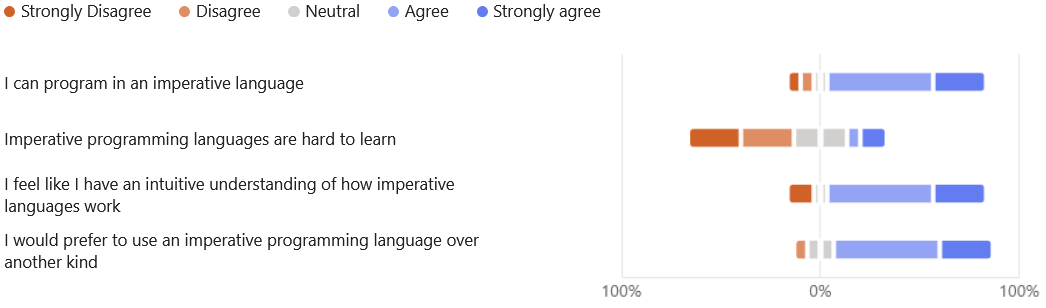
\includegraphics[width=\linewidth]{images/imperative_likert.png}
        \caption{}
        \label{fig:imp_is_easy}
    \end{subfigure}
    
    \begin{subfigure}{\textwidth}
        \centering
        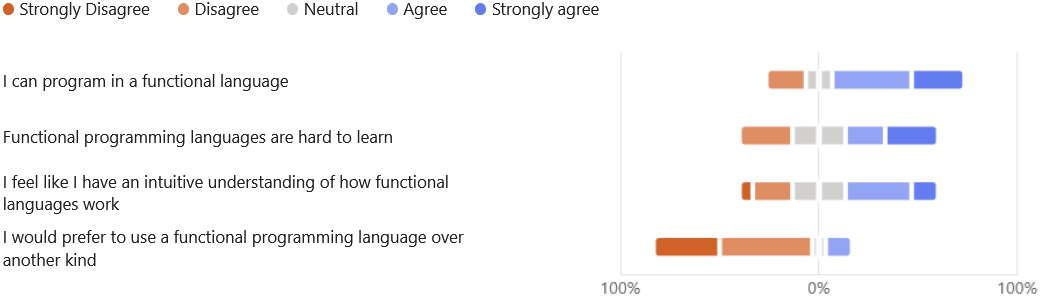
\includegraphics[width=\linewidth]{images/fp_likert.png}
        \caption{}
        \label{fig:fp_is_hard}
    \end{subfigure}
    \caption{The results of a survey performed during the testathon, where a Likert scale was used to gauge 15 participants feelings towards imperative (a) and functional (b) programming languages}
\end{figure*}

For imperative languages, $80\%$ of respondents agreed/strongly agreed that they can program in them, similarly $80\%$ of respondents agreed/strongly agreed that they had an intuitive understanding of them. For functional languages, $66.7\%$ of respondents strongly/agreed that they knew them, but only $47.6\%$ of respondents would agree/strongly agree that they had an intuitive understanding of them. The number of people who claim to know how to program in functional languages is less than imperative, but more striking is the difference in reported `intuition'. 